\documentclass[11pt]{article}

\usepackage{float}
\usepackage{hyperref}
\usepackage{fullpage}
\usepackage{verbatim}
\usepackage{moreverb}
\usepackage{graphicx}
\usepackage{array}
\usepackage{booktabs}
\usepackage{parskip}
\usepackage{tikz}
\usetikzlibrary{arrows,automata, positioning}
\usepackage{minted}
\let\verbatiminput=\verbatimtabinput
\def\verbatimtabsize{4\relax}
\graphicspath{{images/}}

\begin{document}
\title{EECS 151/251A FPGA Lab\\
Lab 6: AC97 (Audio) Controller and FPGA - IC Communication}

\author{Prof. Borivoje Nikolic \\
TA: Vighnesh Iyer \\Department of Electrical Engineering and Computer Sciences\\
College of Engineering, University of California, Berkeley}
\date{}
\maketitle

\tableofcontents

\section{Before You Start This Lab}

These documents will be helpful as you work through this lab.

\begin{enumerate}
	\item \textbf{labs\_fa16/docs/AC97\_Spec.pdf}
	
	The official specification of the AC97 protocol which you will partially implement in this lab. This is a large document but there are only a few sections that are important to us. They will be referenced later in the spec.
	
	\item \textbf{labs\_fa16/docs/AD1981B\_Datasheet.pdf}
	
	The datasheet of the AD1981B AC97 Audio Codec. We will be writing a controller that lives on the FPGA which will communicate with this IC using the AC97 protocol. This IC receives audio data over the AC97 protocol and converts the digital audio data to an analog signal which is sent through the headphone jack.
\end{enumerate}

\textbf{We strongly recommend you read through this entire document before coming to lab.}

\section{Lab Overview}
Run \verb|git pull| in your \textbf{git cloned} \verb|labs_fa16| directory to \textbf{fetch the latest skeleton files for this lab.}

In this lab, we will create a AC97 controller that lives on the FPGA. The controller will interact with an AC97 audio codec IC on the ML505 development board. Your controller will implement a portion of the AC97 protocol that will allow it to send digital audio data and control signals to the IC.

\textbf{This lab will be done in teams of two; it will involve building a peripheral used in the project.}

\section{Introduction to the AC97 Protocol}
AC97 is a protocol which is used for communication between a source/producer of audio data and an audio codec. The audio codec present on the FPGA development board (ML505) is the Analog Devices AD1981B Codec. Our AC97 controller will send digital packets to this codec using the AC97 protocol. The AC97 codec will decode the signals sent to it and send a voltage out through the headphone jack on the back of the ML505 board. You can plug in your headphones and listen to its output.

Refer to the AD1981B Codec datasheet and the official AC97 spec when working through this lab. They are in the \verb|labs_fa16/docs| folder.

\subsection{Protocol Connections}

\begin{figure}[H]
	\begin{center}
		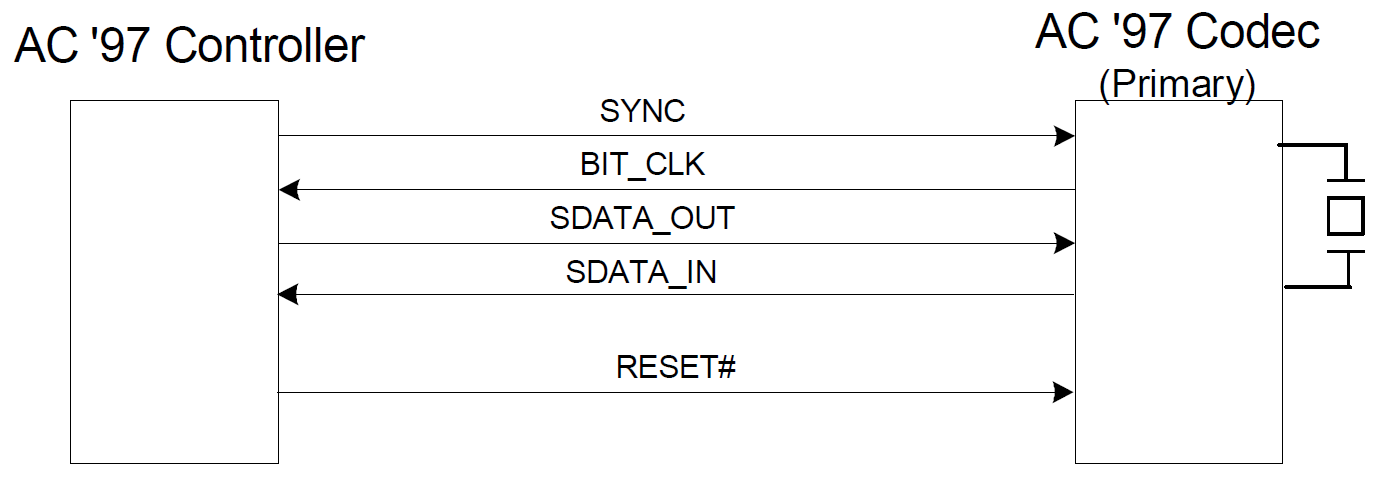
\includegraphics[width=6in]{ac97_connections}
		\caption{Codec - Controller Connections}
	\end{center}
\end{figure}

There are 5 wires involved in the AC97 protocol. They are

\begin{enumerate}
	\item \verb|SYNC| - tells the codec when a frame is about to start
	\item \verb|BIT_CLK| - a clock from the codec which your controller should synchronize its data transfers with
	\item \verb|SDATA_OUT| - the serial line on which your controller transmits data to the codec
	\item \verb|SDATA_IN| - the serial line on which the codec transmits data to your controller (not used in this lab)
	\item \verb|RESET#| - a signal used by your controller to reset the codec
\end{enumerate}

The way in which your controller transmits audio samples (linear PCM) to the codec is through the \verb|SDATA_OUT| wire. There is a specific method of framing the samples so that the codec knows how to read them which is defined by the AC97 spec.

\subsection{How Data is Transmitted}
AC97 is a \textbf{serial interface}: data is transmitted to and from the codec one bit at a time. On every cycle of the AC97 bit clock (\verb|BIT_CLK|), one bit of data is transfered from the AC97 controller (on the FPGA) to the codec over the \verb|SDATA_OUT| wire, and one bit of data is transfered from the codec to the FPGA over the \verb|SDATA_IN| wire.

The constant streams of data passing between the codec and the FPGA are divided into frames. The bit clock is generated by the codec, and runs at 12.288MHz. There are 256 bits per frame, so 48,000 frames are sent per second. This is where the 48kHz sampling rate of the codec comes from. Each frame sent to the codec provides one 20-bit audio sample for each of the DACs in the codec, and each frame sent by the codec provides one 20-bit sample from each of the codec's ADCs.

Frames are divided into twelve slots of 20 bits each, plus a 16-bit tag field, which serves as the frame header. Each slot serves a different purpose and contains various types of data to be sent to the codec. Each slot should be sent with the MSB first going down to the LSB. For example if you were to send \verb|data[19:0]| in slot 1, you would begin by sending \verb|data[19]| and finish by sending \verb|data[0]|.

The start of each frame is indicated by a rising edge of the SYNC signal. The SYNC signal goes high one clock cycle before the first bit of a frame, and goes low at the same time as the last bit of the tag field is sent. The diagrams below will summarize how frames are sent using the AC97 protocol.

\begin{figure}[hbt]
	\begin{center}
		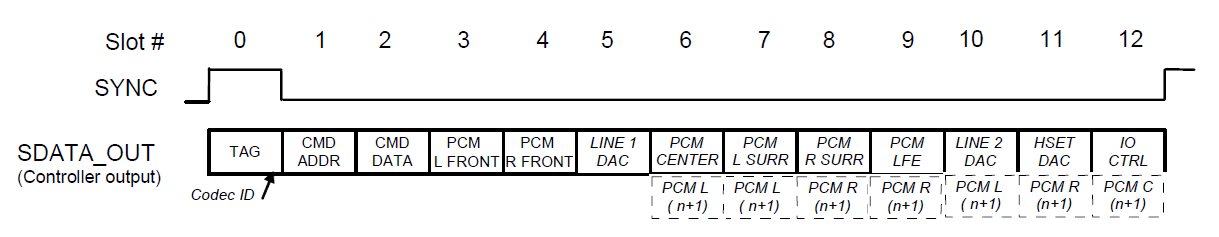
\includegraphics[width=6in]{ac97_framing}
		\caption{Framing for AC97}
	\end{center}
\end{figure}

\begin{figure}[hbt]
	\begin{center}
		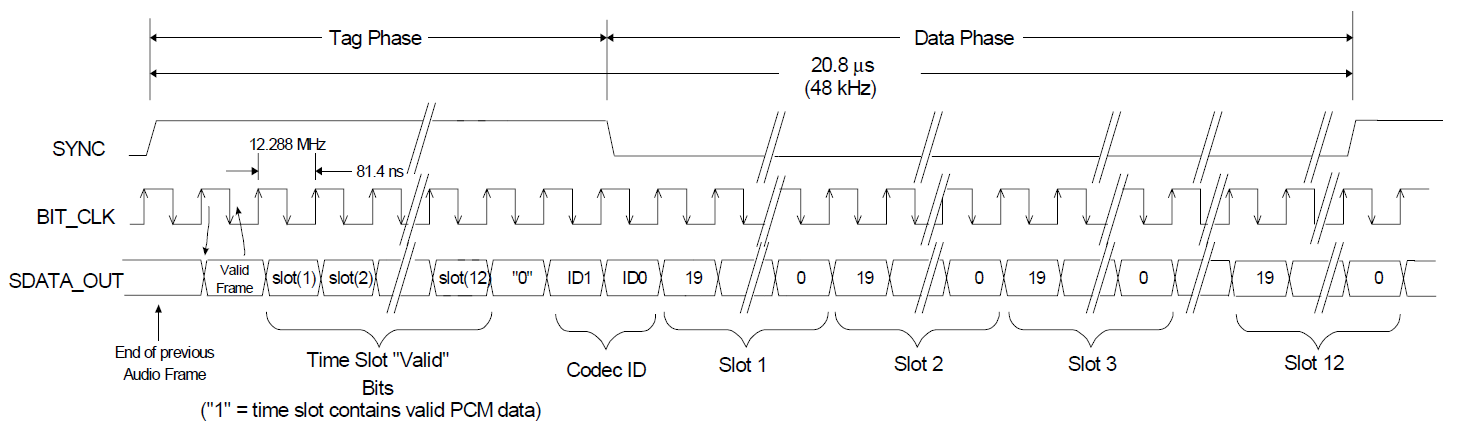
\includegraphics[width=6in]{ac97_framing_detail}
		\caption{Framing for AC97 with Timing Details}
	\end{center}
\end{figure}

\subsection{Sending the Frame Tag (Slot 0)}

The bits in the tag (slot 0) are indicate which, if any, of the other slots in the frame are valid. The tag bits are assigned as follows:

\renewcommand{\arraystretch}{1.1}
\begin{center}
	\begin{tabular}{ | l | l | p{8cm} |}
		\hline
		\textbf{Bit} & \textbf{Description} & \textbf{Value} \\ \hline
		15 & Frame Valid & Should be 1 always  \\ \hline
		14 & Slot 1: Valid Register Address & Should be 1 if we are writing or reading from a control register in the codec  \\ \hline
		13 & Slot 2: Valid Register Data & Should be 1 if we are writing to a control register in the codec \\ \hline
		12 & Slot 3: PCM Left Channel Valid Data & Should be 1 if we have a sample to send to the codec  \\ \hline
		11 & Slot 4: PCM Right Channel Valid Data & Should be 1 if we have a sample to send to the codec  \\ \hline
		10-0 & Etc. Valid Bits & Should be set to 0 \\ \hline		
	\end{tabular}
\end{center}

\subsection{Setting Control Registers With Slots 1 and 2}
After you send the correct tag through \verb|SDATA_OUT|, you will then need to fill slots 1 and 2. These slots contain an address and a value which refer to some control register on the codec IC. The codec contains a multitude of registers which control various features (volume/gain, mute, etc.). Our controller will need to manipulate some registers to unmute the codec and to set the volume appropriately.

\textbf{You should refer to the codec datasheet, specifically the table on page 12} to get the details of these control registers. We have specified below the registers that you will need to manipulate.

\begin{center}
	\begin{tabular}{ | l | l | p{10cm} |}
		\hline
		\textbf{Reg Address} & \textbf{Description} & \textbf{Value} \\ \hline
		0x02 & Master Volume & Should unset the mute bit and set right and left volume \\ \hline
		0x04 & Headphone Volume & Should unset the mute bit and set right and left volume \\ \hline
		0x18 & PCM-Out Volume & Should unset the mute bit and set right and left volume \\ \hline
	\end{tabular}
\end{center}

In \textbf{slot 1}, the command register address needs to be specified as follows in 20 bits.
\begin{enumerate}
	\item \verb|Bit[19]| - Read/Write Command (1 = read, 0 = write)
	\item \verb|Bit[18:12]| - Control Register Address (64 16-bit locations, addressed on even byte boundaries)
	\item \verb|Bit[11:0]| - Set to 0
\end{enumerate}

The first bit (MSB) sampled by AC97 indicates whether the current control transaction in this frame is a read or write operation. The following 7 bit positions communicate the targeted control register address. The trailing 12 bits should be 0.

In \textbf{slot 2}, the command register data needs to be specified as follows in 20 bits:

\begin{enumerate}
	\item \verb|Bit[19:4]| - Control Register Write Data (16 bits)
	\item \verb|Bit[3:0]| - Set to 0
\end{enumerate}

If we are writing data to a register, you must send the data with the MSB first in the first 16 bits of slot 2. If you are reading data, the entire slot 2 must be filled with 0s.

\subsection{Sending Linear PCM (pulse code modulation) Samples in Slots 3 and 4}
The next 2 slots \textbf{(slots 3 and 4)} are used for sending the actual audio samples you want the codec to push to the headphone output. Remember that the samples must be transmitted MSB first and each sample is 20 bits wide. Also note that each sample is a signed integer encoded with 2s complement, so the total range is roughly $\pm 2^{19}$. Each sample represents the amplitude of the audio wave to be played.

Fill the remaining slots \textbf{(slots 5-12)} with all 0s for each 20-bit slot.

\subsection{Codec Timing}
The datasheet is useful for figuring out how the timing works with the codec. Pay close attention to the timing parameters and diagrams on \textbf{pages 6-7 of the datasheet} as your controller needs to be coded with those in mind.

Your controller will need to send bits on the rising edges of \verb|BIT_CLK|, and the codec will sample them on the falling edge of the \verb|BIT_CLK|. Recall, that the \verb|BIT_CLK| is provided by the codec.

\subsubsection{Codec Reset}
Your controller will have to perform a cold reset of the codec when it receives a reset signal from the FPGA board (when you press the \verb|CPU_RESET| button). The cold reset timing is critical, since if your controller doesn't hold the reset properly, the codec may lose its clock.

This timing diagram below is critical to understanding how to reset the codec.

\begin{figure}[hbt]
	\begin{center}
		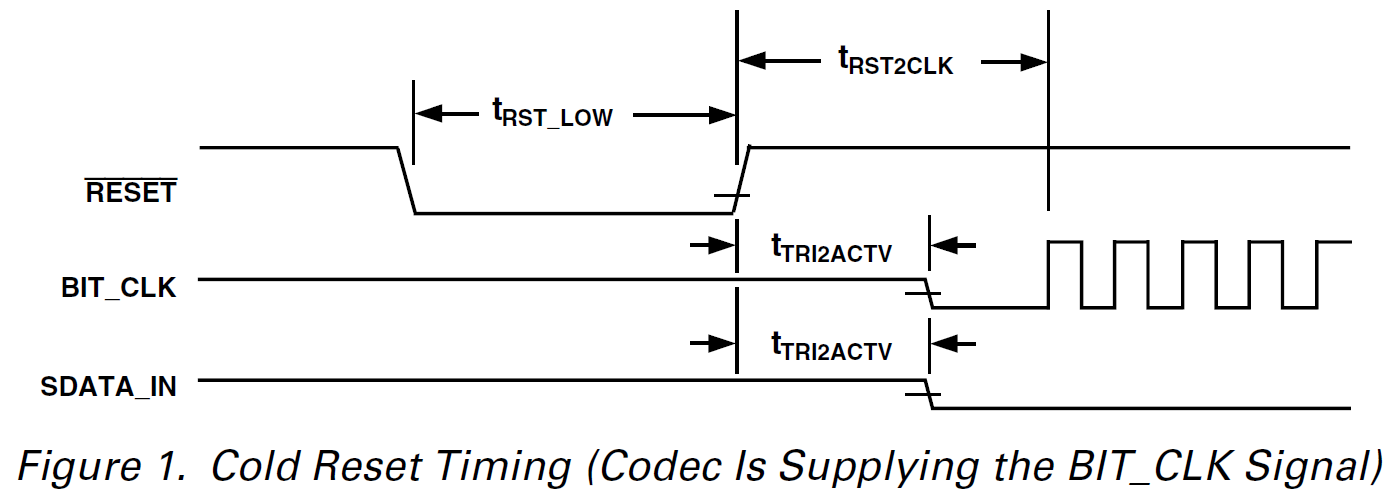
\includegraphics[width=6in]{ac97_codec_timing}
		\caption{Reset Timing Diagram from Datasheet}
	\end{center}
\end{figure}

You will notice from the diagram, that the reset signal that your controller will send to the codec is active low, which means that to assert the reset signal, you have to pull the line low. You will need to pull the reset signal low for at least $t_{RST\_LOW}$ which is defined in the datasheet. While the reset signal is being asserted, the codec will stop producing the \verb|BIT_CLK| and thus you cannot rely on it during reset; you must instead rely on a different clock to time the reset.

Once the reset signal has been asserted for the required time, after a delay of $t_{RST2CLK}$, the \verb|BIT_CLK| will begin to oscillate, after which the controller can begin transmitting frames to the codec. When the codec undergoes a cold reset, all its registers are set to their default values as specified in the datasheet.

\subsubsection{SYNC Signal for Frame Timing}
The codec needs a way to know when a frame is about to begin so that it can interpret its content appropriately. This is done using the \verb|SYNC| signal which is sent from your controller to the codec. You should assert \verb|SYNC| for a total duration of 16 \verb|BIT_CLK|s at the beginning of each audio frame. Refer back to Figure 3 in Section 3.2 to understand how the \verb|SYNC| signal should be asserted with each frame.

\section{Copy Over (Modify) Lab 4 Designs}
You should copy over your lab 4 input processing circuits. Copy over your implementations of \verb|synchronizer.v, debouncer.v, edge_detector.v|, and \verb|rotary_decoder.v|. Then copy over your \verb|tone_generator.v| and \verb|music_streamer.v|. You can directly copy these files over from your \verb|labs_fa16/lab4| directory.

\textbf{If you use the 'rst' input in your synchronizer, debouncer, or edge detector, you should NOT use it for this lab. Instead of using a reset signal to initialize your module's registers, use a reg assignment so that your simulations continue to work, like this:}

\begin{minted}{verilog}
	reg [width-1:0] prev_values = 0;
\end{minted}

You might have to add this code to reset the 2D saturating counter register in your debouncer if you are getting Xs in simulation:

\begin{minted}{verilog}
    initial begin:INITIALIZE_SAT_COUNTER
	    integer k;
	    for (k = 0; k < width; k = k + 1) begin
		    saturating_counter[k] <= 0;
	    end
    end
\end{minted}

{\footnotesize The reason for this is due to a feedback loop from the edge detector's pulse from a reset button press back to the debouncer, resetting the saturating counter and triggering another reset pulse. This was OK for the previous labs, but the AC97 codec is very sensitive to being reset frequently.}

\section{Building the AC97 Controller}

Open up \verb|labs_fa16/lab6/src/ac97_controller.v|. You will be implementing your AC97 controller in this module.

\subsection{I/O Ports}
\begin{itemize}
	\item \verb|sdata_in, bit_clk, sdata_out, sync, reset_b| 
	
	These are the signals comprising the AC97 protocol. They behave as mentioned in the previous section. The \verb|reset_b| signal flows directly to the AC97 codec and the \verb|sdata_out, sync| signals go through a register in \verb|ml505top| clocked by the \verb|bit_clk| before going to the AC97 codec. The \verb|reset_b| signal is an active low reset, which means that to assert the reset to the codec, you must pull the signal low.
	
	\item \verb|system_clock, system_reset|
	
	The \verb|system_clock| is a 33Mhz clock that will continuously operate. The \verb|system_reset| is a 1 clock cycle reset pulse that is generated when you press the \verb|CPU_RESET| button. The \verb|system_reset| comes from a synchronizer $\rightarrow$ debouncer $\rightarrow$ edge detector chain.
	
	\item \verb|volume_control [3:0]|
	
	This input will be explained in more detail in the Volume Control section. This signal is tied to the GPIO DIP switches 3, 4, 5, 6.
	
	\item \verb|square_wave|
	
	This input comes from your \verb|tone_generator| and is either 0 or 1, indicating the state of the square wave to play. Your AC97 controller will output this square wave input to the codec using the AC97 protocol.
\end{itemize}

\subsection{General Operation}

In the general case, the \verb|bit_clk| will operate at its specified frequency. Your controller's job is to send AC97 frames to the codec. It will need to set \verb|sdata_out| and \verb|sync| in accordance to the AC97 specification.

For sending data to the codec, the AC97 protocol defines 2 20-bit slots for PCM data per AC97 frame. The data you send corresponds to digital inputs to the DACs on the codec. These slots should be filled with -250000 or 250000 based on whether the \verb|square_wave| input signal is high or low. Since we are sending signed PCM samples to the codec, you will need a way of holding a signed number. To do this in Verilog, we can use the 'signed' keyword on a wire or reg net as such:

\begin{minted}{verilog}
	wire signed [19:0] pcm_data;
	assign pcm_data = -20'd250000;
\end{minted}

You are also in charge of setting the three previously specified registers of the AC97 codec so that the volume level is set properly and so that the output is unmuted. It is recommended that you write to these registers in a loop so that you are performing a register write every frame; this will make your controller simpler.

\subsection{Resetting the Codec}
When we assert the \verb|reset_b| signal to the codec, the \verb|bit_clk| stops oscillating and only begins again after the \verb|reset_b| signal has been deasserted. However, we need to precisely time how long the reset signal is asserted. To do this, we will use the \verb|system_clock| which is always oscillating, and use the \verb|system_reset| input to trigger a codec reset.

You should read the datasheet for the codec and understand how to reset it. Make sure you reset the codec for the required amount of time. 

\textbf{Be careful, however, since resetting the codec too frequently or for too long can cause the codec to lose its clock and stop operating.} If this happens to you, you can recover by re-running \verb|make impact|.

\subsection{Resetting Controller Registers}
When the \verb|system_reset| is asserted, you should only touch one register, which is your reset clock counter that times the reset. Other registers that are modified by the posedge of the \verb|bit_clk| shouldn't be touched.

In order to get simulation working and your other design registers (frame shift register, frame counter, etc.) in your design to a default state, you should use reg assignments.

\begin{minted}{verilog}
	reg [255:0] frame_to_send = 256'd0;
\end{minted}

\subsection{Clock Crossing}
The design of the AC97 controller is tricky since it involves 2 clocks. Generally, you do not want registers that are set by one clock, to be used in combinational logic and then registered by another clock. However, we have that circumstance in this design.

Our \verb|music_streamer| and \verb|tone_generator| are being clocked by the 33 Mhz system clock, while the logic that sends data over \verb|sdata_out| is being clocked by the \verb|bit_clk|. Ordinarily, this would pose a problem, since the \verb|square_wave| register is being set in the system clock domain, and its value is being read, used, and registered in the \verb|bit_clk| domain. 

However, in this particular case, since the \verb|square_wave| register updates are so infrequent with respect to both the clocks, and a brief glitch in the square wave would make hardly any impact on the audio output, we can use the \verb|square_wave| value in the \verb|bit_clk| domain without much worry.

\textbf{This happy circumstance will not persist into the project.} In the project you will design a more sophisticated synchronization scheme to move multiple bits in parallel from the system clock domain to the \verb|bit_clk| domain using an async FIFO.

\subsection{Volume Control}
Your AC97 controller needs to unmute and set the volume of the audio output using three registers in the codec. These registers should be set as such (look at the datasheet for the details):

\begin{center}
	\begin{tabular}{ | l | l | p{8cm} |}
		\hline
		\textbf{Reg Address} & \textbf{Description} & \textbf{Value} \\ \hline
		0x02 & Master Volume & Unmute and set R/L attenuations equal to \verb|{1'b1, volume_control}| \\ \hline
		0x04 & Headphone Volume & Unmute and set R/L attenuations equal to \verb|{1'b1, volume_control}| \\ \hline
		0x18 & PCM-Out Volume & Unmute and set R/L gain to 0dB \\ \hline
	\end{tabular}
\end{center}

\textbf{WARNING: If sufficient attenuation isn't applied, the codec may supply too much voltage to your headphones and destroy them. Check with the TA if you are unsure about the values written to the registers.}

\subsection{SYNC Signal Timing}
As a note, if you create registers for the \verb|sync| and \verb|sdata_out| signals, make sure that they are both registered the same number of times and march in line.

You will need to make sure the \verb|sync| signal is applied properly as you send each AC97 frame. Refer to Figure 3 in Section 3.2 for details. You should raise the \verb|sync| signal on the last bit of the previous frame and hold it high until bit 15 has been sent of the next frame.

\subsection{Testing in Simulation}
To test our AC97 controller, we will be using a \textbf{block-level testbench}. This testbench will simulate our AC97 controller in isolation to see if it performs to spec.

The source for this testbench is \verb|lab6/src/ac97_controller_testbench.v|. Run the testbench as usual by running \verb|make| in the \verb|lab6/sim| directory. This testbench isn't self checking so you should look at the Verilog file and manually inspect the output waveform to verify that all specifications are met. You should extend the testbench so that it sends more stimulus to the AC97 controller (like changing the volume).

You should make sure that ALL the signals in your AC97 controller are well defined (not X) for the entirety of the simulation.

\section{Connect the music\_streamer and tone\_generator}

\subsection{Testing in Simulation}
We previously used a block-level testbench to just test the AC97 controller in isolation. Now we will use a \textbf{system/chip-level testbench} to test our entire system at a higher level. This dichotomy is similar to the difference between unit tests and integration tests in software.

Take a look at the source for this testbench in \verb|lab6/src/system_testbench.v|. You will notice that instead of instantiating the AC97 controller, it instantiates \verb|ml505top|. Now, the stimulus that we supply to our DUT represent signals coming into the FPGA.

This testbench will simulate the entire system which connects your AC97 controller to the \verb|tone_generator|, which is connected to the \verb|music_streamer|, which has connections from your input conditioning circuits (synchronizer, debouncer, edge detector, rotary decoder). This testbench isn't self-checking either, so you should add stimulus to the DUT to make it respond in some way and see that it is reflected in the waveform.

You should make sure that ALL of the signals in your entire system are well defined (not X) for the entirety of the simulation.

\section{Try it on the FPGA!}
With both simulations indicating that everything seems to be working, run \verb|make| and \verb|make impact| from the \verb|lab6| directory. When your design is on the FPGA, your music streamer FSM from Lab 4 should still work as usual. By turning on the 1st and last DIP switches, the piezo output will be enabled. But now, as long as the 1st DIP switch is turned on, you can plug in a pair of headphones to listen to the output of the music streamer FSM. 

You can use DIP switches 3-6 to change the volume of the audio output. Keep in mind that making all the switches high will give you the max attenuation, which corresponds to the quietest volume.

\section{Conclusion + Checkoff}
You are done with lab 6! Please write down any and all feedback and criticism of this lab and share it with the TA. This is a brand new lab and we welcome everyone's input so that it can be improved.

The differences between a block and system level testbench will be critical in the testing of your project. You will use both types of testbenches extensively to verify correct behavior of all the modules you write.

\subsection{Checkoff Tasks}

\begin{enumerate}
	\item Show the TA your working AC97 controller by demonstrating the state machine in the \verb|music_streamer| working and sending audio to the AC97 codec.
\end{enumerate}

\end{document}